%----------------------------------------------------------------------------
\chapter{Mérési feladatok}\label{sect:LatexTools}
%----------------------------------------------------------------------------
%
%\begin{figure}[!ht]
%	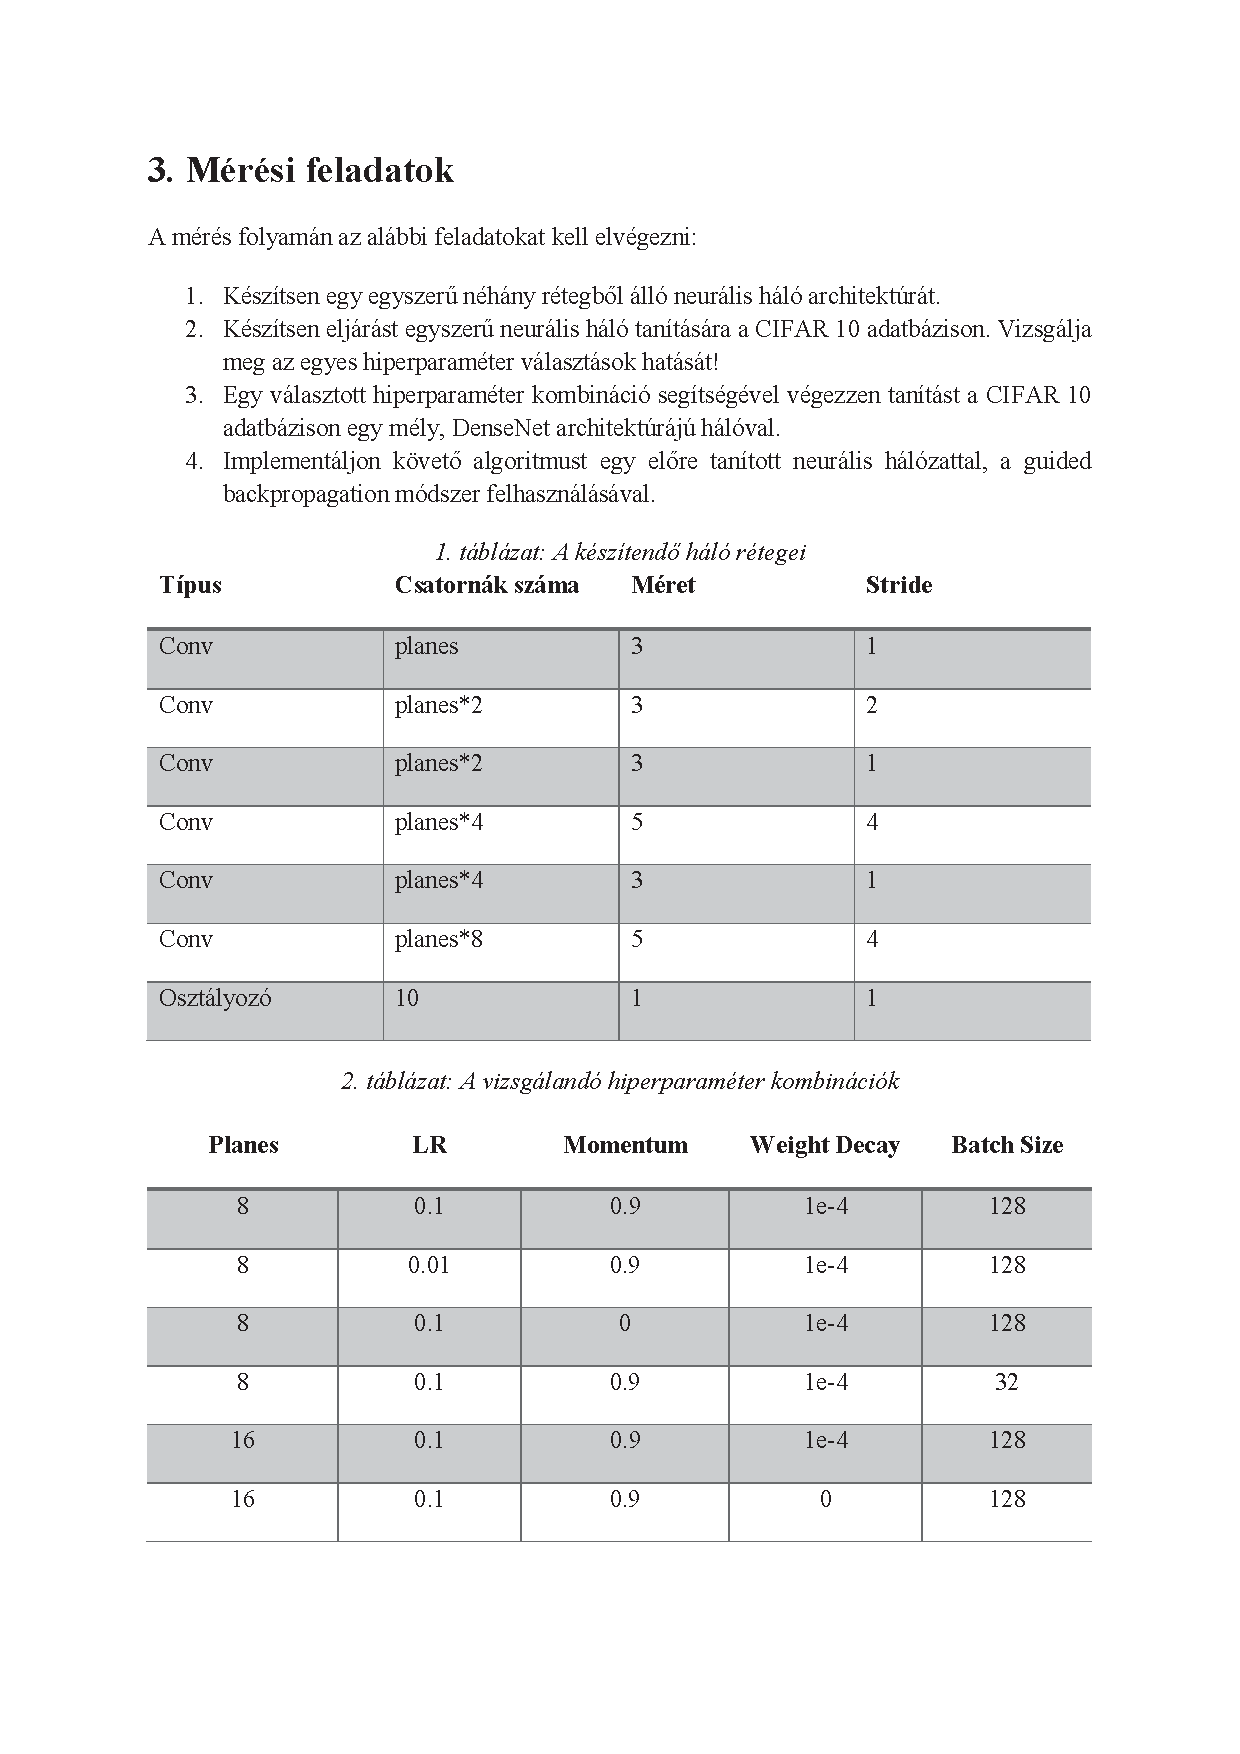
\includegraphics[trim = 25mm 210mm 20mm 33mm,clip, width=150mm,keepaspectratio]{figures/feladatok_m07.pdf}
%	\label{fig:Road-of-a-char}
%\end{figure}

A mérés folyamán az alábbi feladatokat kell elvégezni:
\begin{enumerate}
	\item Készítsen eljárást a sávokat jelentő élek detektálására! Az éldetektálás során kapott gradienseket szűrje nagyság és irány alapján, valamint végezzen szín alapú szűrést is!
	\item Torzítsa a képet perspektív transzformáció segítségével úgy, hogy a sávok párhuzamosak legyenek, majd határozza meg a sávok helyzetét!
	\item Készítsen robusztus becslőt a sávok görbületének, az autó helyzetének és ez utóbbi változásának meghatározására!
	\item Valósítson meg egy sávtartó algoritmust egyszerű fuzzy irányítás segítségével!	
	\item Ellenőrizze az algoritmus helyes működését előre felvett videófelvételek segítségével!
\end{enumerate}
